\section{Results}

\begin{figure*}[!t]
	\centering
	%	\Large{Average performance on different tournament size - Gallagher's Gaussian 21-hi Peaks Function}
	\begin{subfigure}[b]{0.33\textwidth}
		\centering
		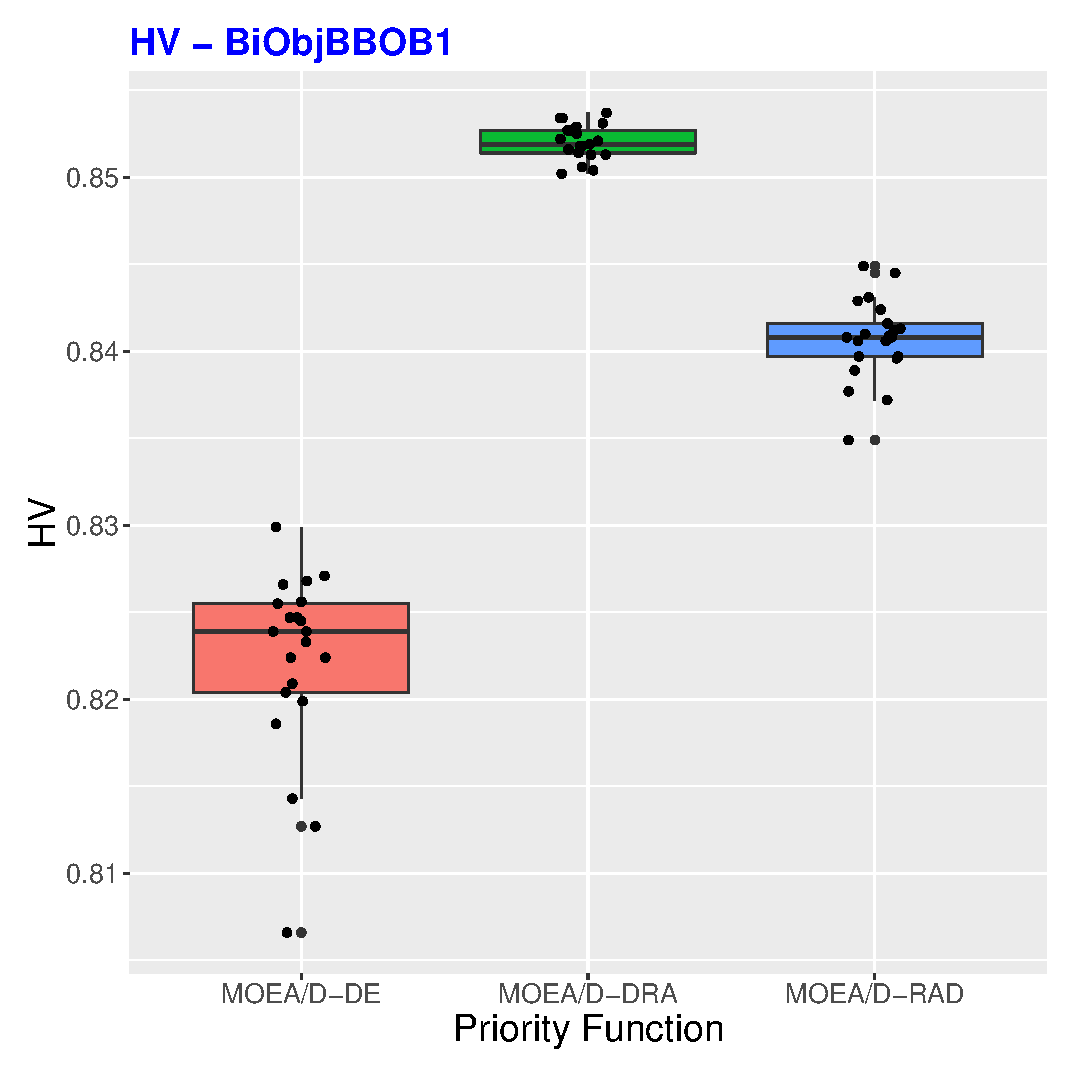
\includegraphics[width=1\textwidth, height=1\textwidth]{img/BiObjBBOB1_HV.eps}
		%	\caption{HV - UF3}
	\end{subfigure}
	\begin{subfigure}[b]{0.33\textwidth}
		\centering
		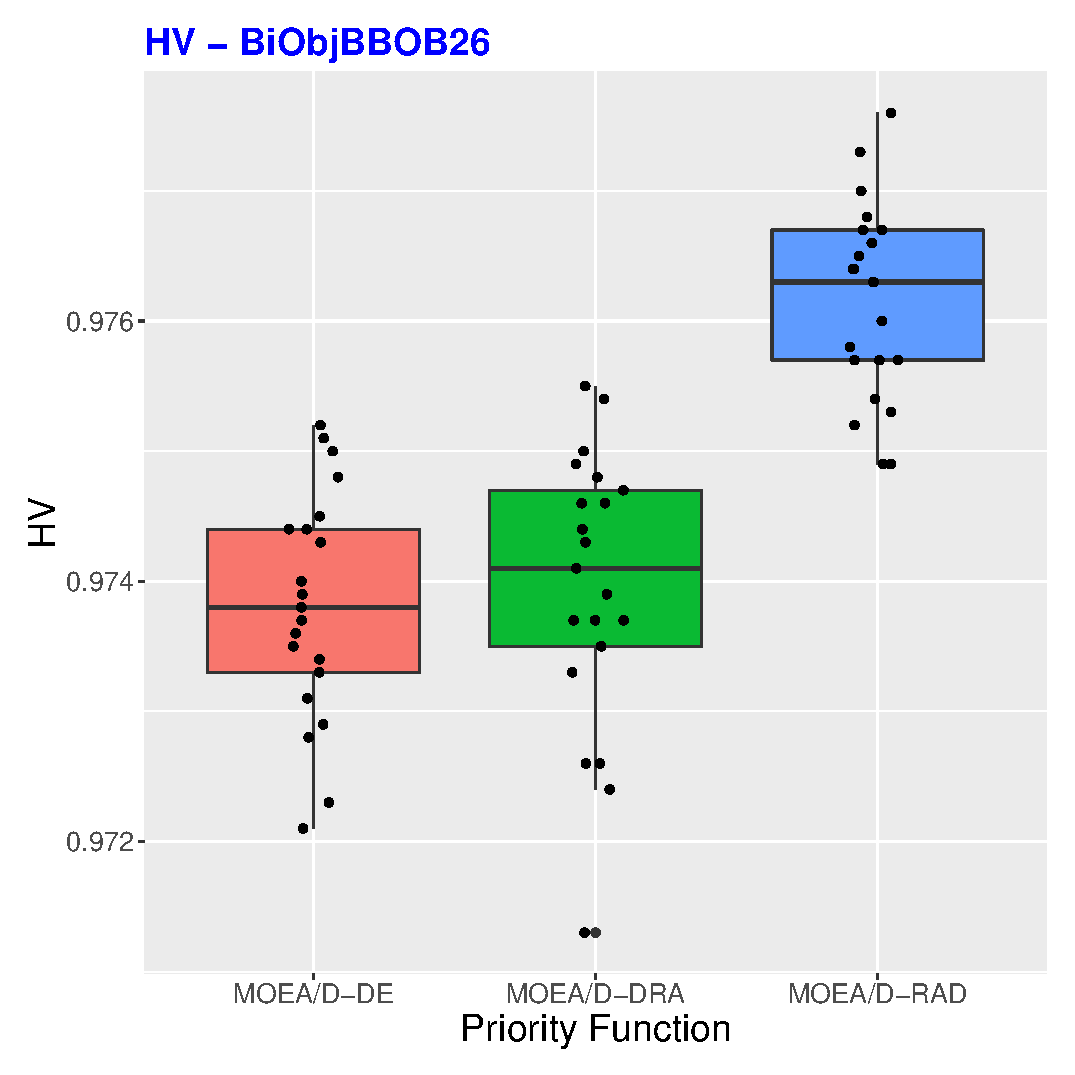
\includegraphics[width=1\textwidth, height=1\textwidth]{img/BiObjBBOB26_HV.eps}
		%	\caption{HV - UF8}
	\end{subfigure}
	\begin{subfigure}[b]{0.33\textwidth}
		\centering
		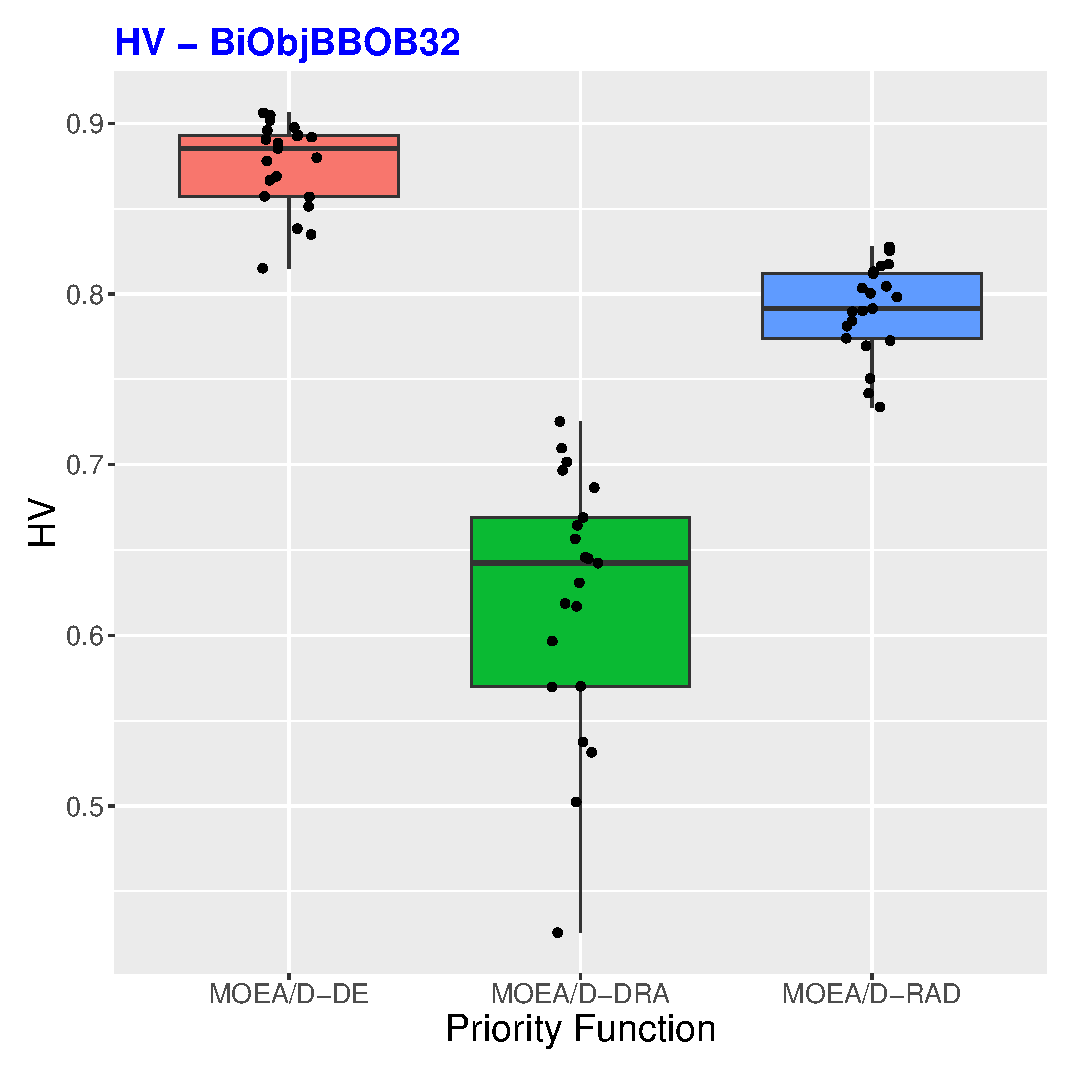
\includegraphics[width=1\textwidth, height=1\textwidth]{img/BiObjBBOB32_HV.eps}
		%	\caption{HV - DTLZ4}
	\end{subfigure}
	\caption{Box plot of HV values on  bbob-biobj-1,  bbob-biobj-26 and  bbob-biobj-32 (Higher values are better).}
	\label{HVS}
\end{figure*}

\begin{figure*}[!t]
	\centering
	%	\Large{Average performance on different tournament size - Gallagher's Gaussian 21-hi Peaks Function}
	\begin{subfigure}[b]{0.33\textwidth}
		\centering
		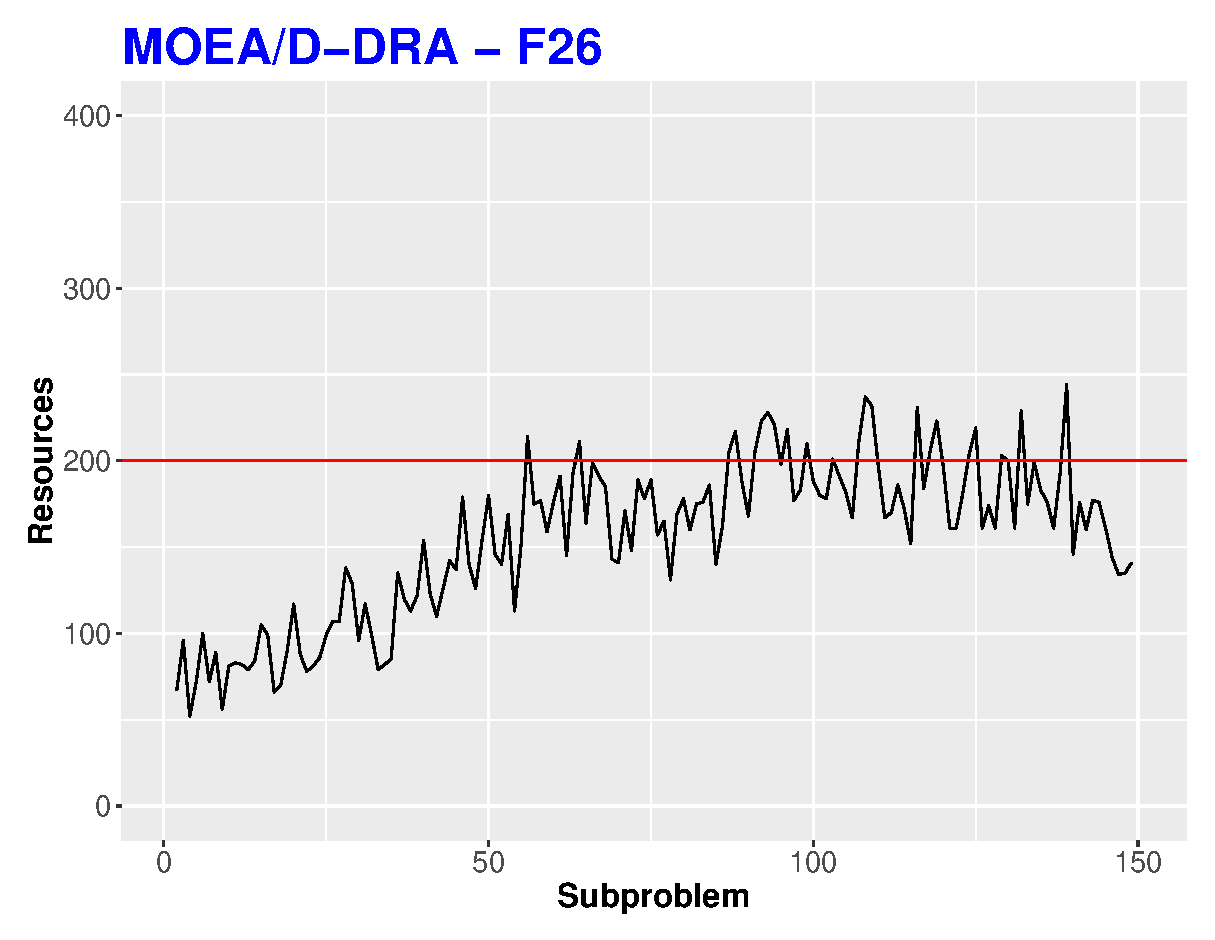
\includegraphics[width=1\textwidth, height=0.8\textwidth]{img/RA-DRA-26.eps}
	\end{subfigure}
	\begin{subfigure}[b]{0.33\textwidth}
		\centering
		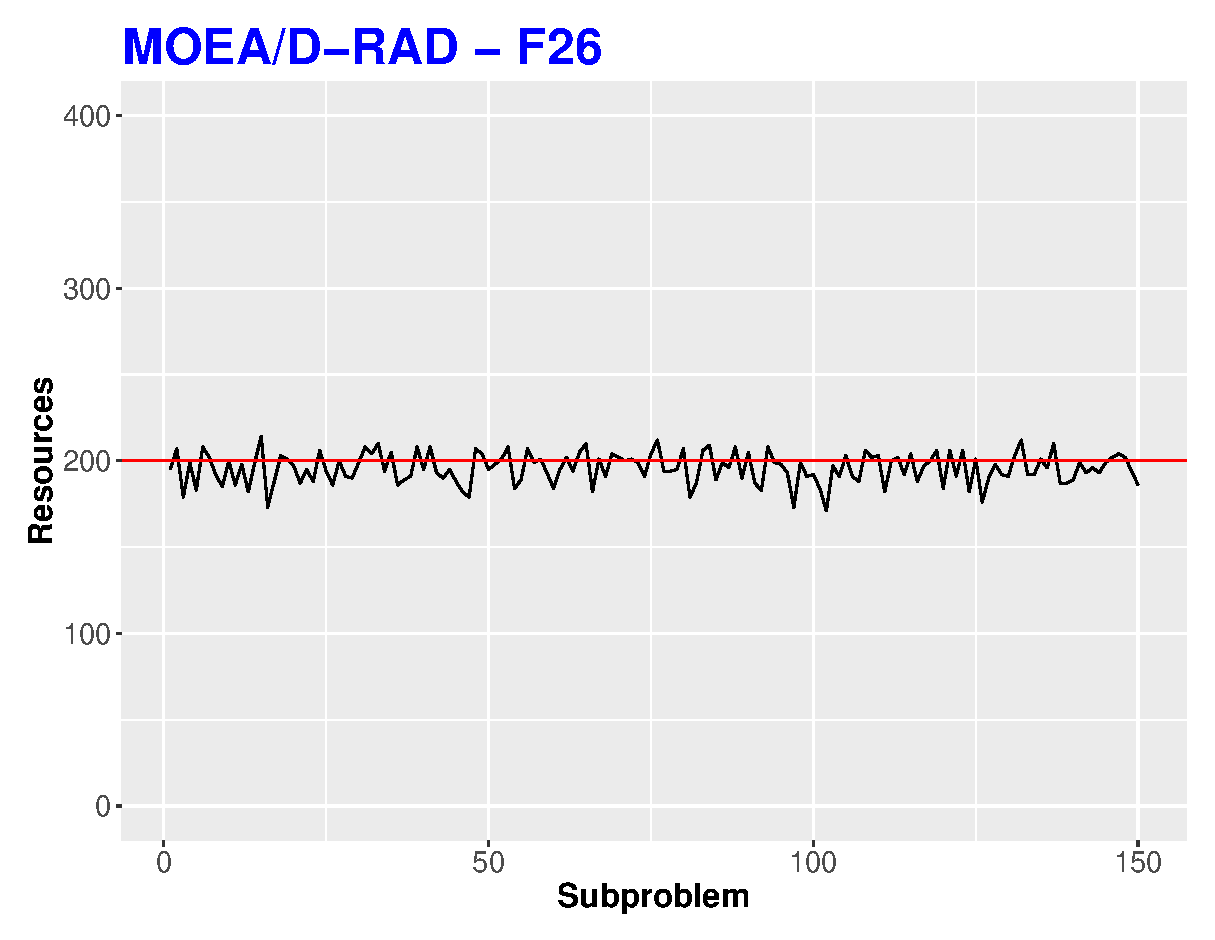
\includegraphics[width=1\textwidth, height=0.8\textwidth]{img/RA-RAD-26.eps}
	\end{subfigure}
	\caption{Resource Allocation by subproblem - The red line indicates the default amount of resource for each problem, i.e., with no priority function.}
	\label{RAs1}
\end{figure*}

\begin{figure*}[!t]
	\centering
	\begin{subfigure}[b]{0.33\textwidth}
		\centering
		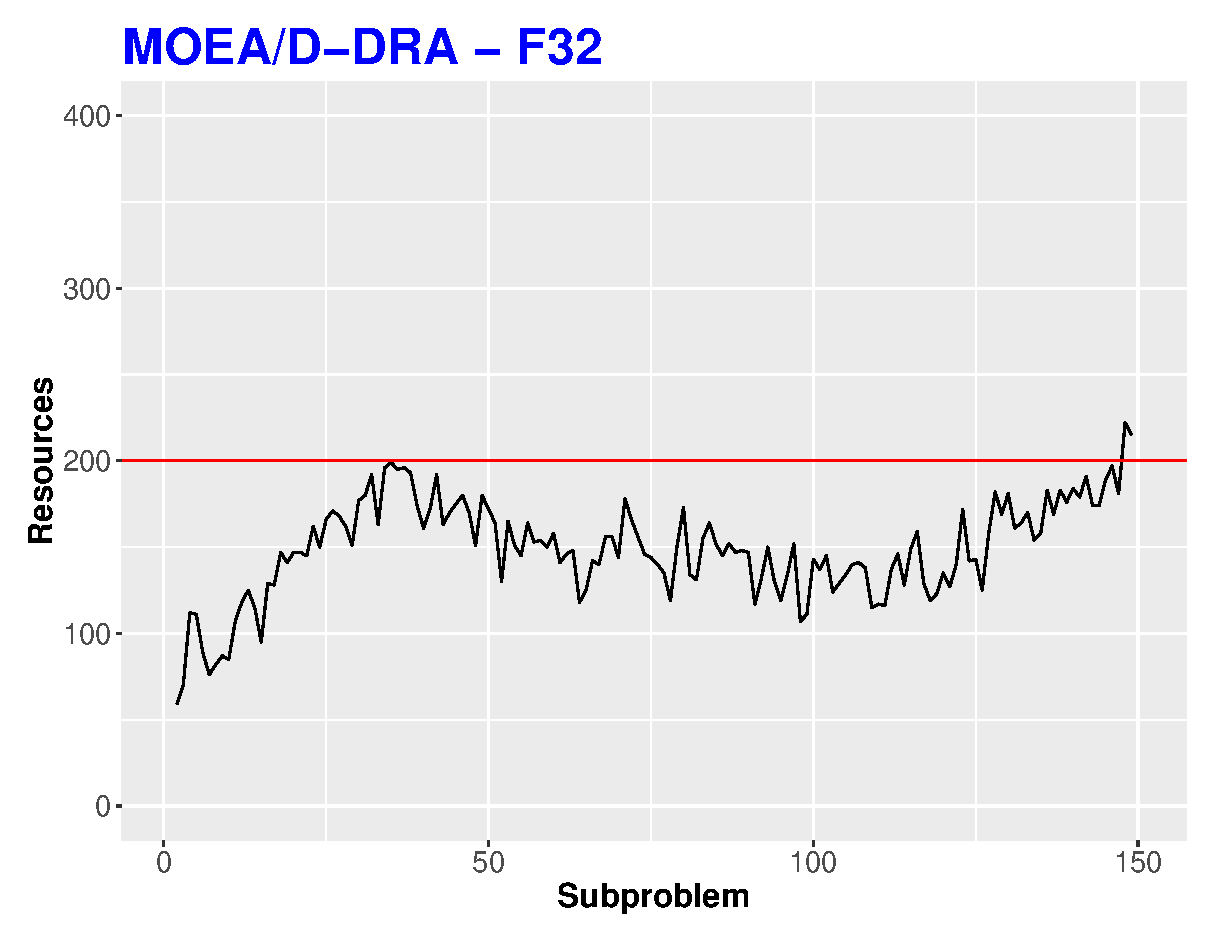
\includegraphics[width=1\textwidth, height=0.8\textwidth]{img/RA-DRA-32.eps}
	\end{subfigure}
	\begin{subfigure}[b]{0.33\textwidth}
		\centering
		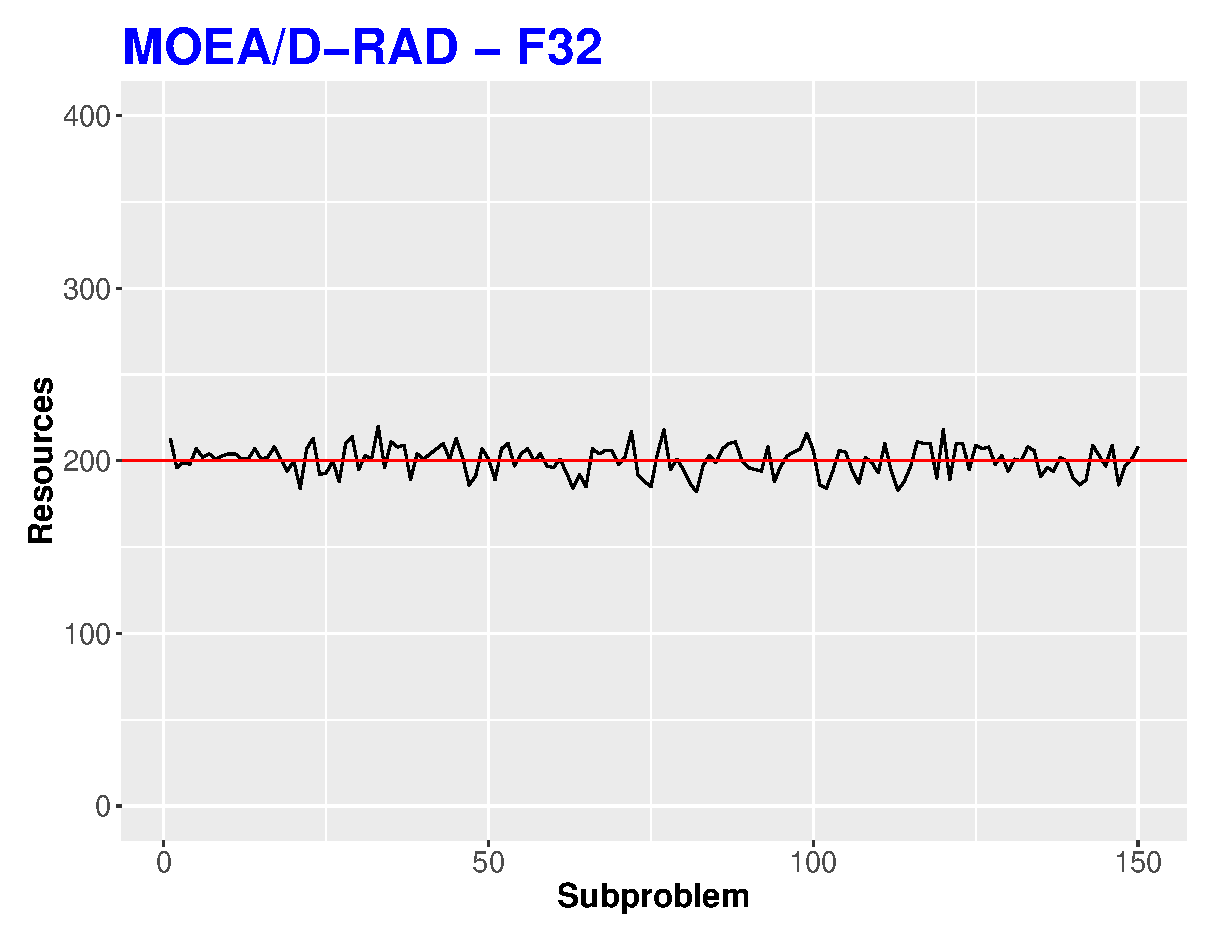
\includegraphics[width=1\textwidth, height=0.8\textwidth]{img/RA-RAD-32.eps}
	\end{subfigure}
	\caption{Resource Allocation by subproblem - The red line indicates the default amount of resource for each problem, i.e., with no priority function.}
	\label{RAs2}
\end{figure*}



\ref{HVS} shows the boxplots of the hypervolume values obtained by the three methods
on functions F26, F1 and F32 of bbob-biobj. F26 is an example of a moderate and
weakly structured function (group 9), where MOEA/D-RAD performed best. F1  is a
separable and separable function (group 1), where MOEA/D-DRA performed best, and
F32 is a moderate and multi-modal function (group 8), where MOEA/D-DE performed
.

\ref{stats} gives us a general view of these results over all functions and
function groups. In general, MOEA/D-RAD performed better than the other methods
(or second best) in terms of hypervolume. This ranking is reinforced by a
Pairwise Wilcoxon Rank Test over the entire experiment~(\ref{statistics}).

However, a post-hoc analysis of these results focusing on the function groups
suggests some interesting properties of the three methods. We observe that
MOEA/D-RAD was specially successful for function groups that included
moderate-conditioned or weakly-structured functions (groups 2, 5, 6, 7, 8, 9, 12 and
15, shaded in \ref{stats}), and performed slightly worse for groups including
multi-modal functions (groups 4, 8, 11, 13 and 14). In particular, we find it  very
interesting that MOEA/D-DE without priority performed better in the multi-modal
groups. This post-hoc analysis suggests a follow up experiment to confirm this
observations.

\subsection{Proportion of Non-dominated Solutions}

Another difference that we see among the algorithms  is the proportion of non
dominated solutions. The results on the~\ref{stats} indicate that MOEA/D-DRA
leads to the highest rate of non-dominated solutions in the final solution set,
followed by MOEA/D-RAD. In general, both substantially improve this proportion
over the results of MOEA/D-DE.  It seems that there is no relation between
hypervolume performance and the proportion of non-dominated solutions.


\subsection{Resource Allocation}


\ref{RAs1} and \ref{RAs2} illustrate the amount resource allocated by MOEA/D-DRA
and MOEA/D-RAD to each subproblem on problems F26 and F32. MOEA/D-DE is
not included since it does not perform resource allocation.

These figures show how the choice of priority function influences the
resource allocation. The resource allocation by MOEA/D-DRA is much more
adaptive to each problem, while the resource allocation done by
MOEA/D-RAD is more conservative and uniform.

However, even though the resource allocation behavior seen in these figures
may seem limited, it is clear from \ref{stats} that it has a deep impact on
the performance of the algorithm.

\input{51_tables.tex}
